\section{Capitulo 4: Fundamentos teoricos de la computación distriuida}
\subsection{Historias Causales}
Las \textbf{Historias causales} permiten detectar si existe \textcolor{red}{\textbf{Concurrencia}} o \textcolor{red}{\textbf{Causalidad}} entre dos eventos

\begin{center}
    $\subset$ : \textbf{Contenido} $\Rightarrow$ : $A=\{1,2\}$ y $B=\big\{\underbrace{1,2}_{\textcolor{red}{\textbf{A}}},3\big\}$ podemos decir que A $\subset$ B
\end{center}

de lo antes definido tenemos lo siguiente:

\begin{itemize}
    \item \[ \forall e, e' \in E, e \neq e' : [e' \rightarrow e] \Leftrightarrow H(e') \subset H(e) \]
    Esto se puede traducir como: \textcolor{red}{Si $e'$ ocurre antes que $e$, entonces $H(e')$ es un subconjunto de $H(e)$}.

    \item \[ \forall e, e' \in E, e \neq e' : [e' \parallel e] \Leftrightarrow [H(e') \nsubseteq H(e)] \land [H(e) \nsubseteq H(e')] \]
    Esto se lee como: \textcolor{red}{Si $e'$ es concurrente con $e$, entonces $H(e')$ no es un subconjunto de $H(e)$ y $H(e)$ no es subconjunto de $H(e')$}.
\end{itemize}

\subsection{Relojes vectoriales}
Para los relojes vectoriales definiremos la siguiente estructura para el un proceso $P_i$, para n procesos
\[
   \left[ \mathit{Vc}[1], \mathit{Vc}[2], \dots, \mathit{Vc}[i], \dots, \mathit{Vc}[n] \right]
\]

Donde cada indice esta asociado a un proceso $P_i$. De los relojes vectoriales sabemos que $\forall e \in E$: Vc(e) representa H(e).

Continuando, los procesos irán aumentando de la sigueinte forma:

Para \textcolor{red}{\textbf{eventos locales} del proceso $P_i$}:
\begin{enumerate}[label=\textbf{Paso \arabic*:}]
    \item :\\
    Se suma 1 al Vc($e_i$)[i], vale decir que le sumamos 1 a la marca del proceso i
    \item :\\
    Asignarle el valor anterior al resto de los otros procesos, al nuevo evento

    \[
\textcolor{green!50!black}{
  \left[ 
    \mathit{Vc}[1], \mathit{Vc}[2], \dots, 
  }
\textcolor{black}{
    \mathit{Vc}[i]
}
\textcolor{green!50!black}{
    , \dots, \mathit{Vc}[n]
  \right]
}
\]

donde los indices en verde, se mantendran iguales para el evento local.\\
\end{enumerate}

Resultando Finalmente en el siguiente vector para $P_i$

\[
\textcolor{green!50!black}{
  \left[ 
    \mathit{Vc}[1], \mathit{Vc}[2], \dots, 
  }
\textcolor{black}{
    \mathit{Vc}[i] + 1
}
\textcolor{green!50!black}{
    , \dots, \mathit{Vc}[n]
  \right]
}
\]

Para mensajes entre procesos, solo se modifica la marca del proceso que esta mandando el mensaje, por ejemplo, si $P_i$ manda un mensaje a $P_j$, se modifica la marca del vector $P_j$ asociada a $P_i$.

\subsubsection{Propiedades de los rejoles vectoriales}

Lo siguiente que denotameros es \textcolor{red}{\textbf{condición fuerte de un reloj en sistemas distribuidos}} se refiere a la capacidad de determinar de forma bidireccional si un evento precede causalmente a otro, permitiendo un ordenamiento total o casi total de los eventos en el sistema.
\begin{enumerate}
  \item Relación de igualdad:
  \[
  V=V' \equiv  [\forall k: V[k]=V'[K]]
  \]
  \item Relación de orden: 
  \[
  V<V' \equiv [V \neq V'] \land [\forall k: V[k] \leq V'[k]]
  \]
  \item Condición fuerte:
  \[
    e \rightarrow e' \equiv VC(e) < VC(e')
  \]
  \[
      e || e' \equiv \lnot [VC(e)<VC(e')]\land \lnot[VC(e')<VC(e)]
  \]
\end{enumerate}

El  numero de eventos precedentes es equivalente a la suma del vector completo, menos el evento mismo.

La propiedad de detección de apertura nos permite a un proceso $P_j$ detectar que existe un evento e' que ocurre en otro $P_i$ despues de un evento $e_i$ ya conocido por $P_j$. Notese además que los relojes vectoriales tienen la capacidad de \textbf{detectar causalidad, concurrencia, coordinacion centralizada y es tolerante a fallos}. Sin embargo tiene limitaciones, como, \textbf{overhead, complejidad (más complejo que lamport), si bien dijimos que tolera fallas, es deficiente ante fallas bizantinas y sistemas altamente dinamicos (con una entrada y salida de procesos, dado que se tiene que redimencionar el vector)}

\subsection{Monitoreo de una computación distribuida}

Una \textbf{observación valida} si implica una relación causal, deberia estar ordenada, caso contrario, no (esta se podria ver de cualquer forma) 

  \begin{figure}[H]
    \centering
    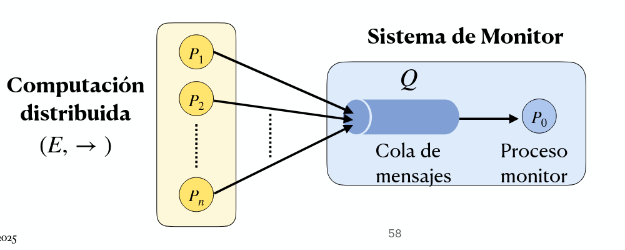
\includegraphics[width=0.5\linewidth]{img/Monitoreo_computacion_distribuida.png}
    \caption{Monitoreo de computacion distribuida}\label{fig:1760794290290}
  \end{figure}

La cola observada en la figura anterior, es la encargada de generar las observaciones validas.

Para entregas causales tenemos las siguientes condiciones:

\textbf{Condición FIFO:}
\begin{figure}[!ht]
\centering
\begin{circuitikz}[scale=1.2, transform shape]
\tikzset{every node/.style={font=\small}}

% Línea principal
\draw (0,0) -- (6,0);

% Nodos
\node[circ] (a) at (0.5,0) {};
\node[circ] (b) at (3,0) {};
\node[circ] (c) at (5.5,0) {};

% Etiquetas de eventos
\node[below=2pt] at (a) {$e_{i,k}$};
\node[below=2pt] at (b) {$e_{i,k+1}$};
\node[below=2pt] at (c) {$e_{i,k+2}$};

% Flechas verdes ("Bien")
\draw [color={rgb,255:red,38; green,162; blue,105}, very thick, ->, >=Stealth] (0.7,-0.4) -- (2.8,-0.4);
\draw [color={rgb,255:red,38; green,162; blue,105}, very thick, ->, >=Stealth] (3.2,-0.4) -- (5.3,-0.4);
\node[color={rgb,255:red,38; green,162; blue,105}, font=\Large] at (3,-1) {Bien};

% Flechas rojas ("Mal")
\draw [color={rgb,255:red,224; green,27; blue,36}, very thick, ->, >=Stealth] (0.5,0.5) -- (5.5,0.5);
\draw [color={rgb,255:red,224; green,27; blue,36}, very thick] (0.5,0) -- (0.5,0.5);
\draw [color={rgb,255:red,224; green,27; blue,36}, very thick] (5.5,0.5) -- (5.5,0);
\node[color={rgb,255:red,224; green,27; blue,36}, font=\Large] at (3,0.9) {Mal};

\end{circuitikz}
\caption{Ejemplo de relaciones entre eventos}
\label{fig:relaciones-eventos}
\end{figure}

Las lineas verdes hacen el flujo de izquierda a derecha que representa una correcta contición FIFO, mientras que las rojas omiten el evento $e_{i,k+1}$ lo cual muestra una incorrecta condición fifo.  \\


\textbf{Condición de entrega causal:} Si yo tengo un mensaje de J, para ver que no exista un mensaje de otro proceso, se compara lo siguiente
\[
  \forall k , i \neq j : Vc_i(m')[k] \geq Vc_j(m)[k]
\]
\subsubsection*{Visualización del algoritmo de entrega causal}

\begin{figure}[H]
  \centering
  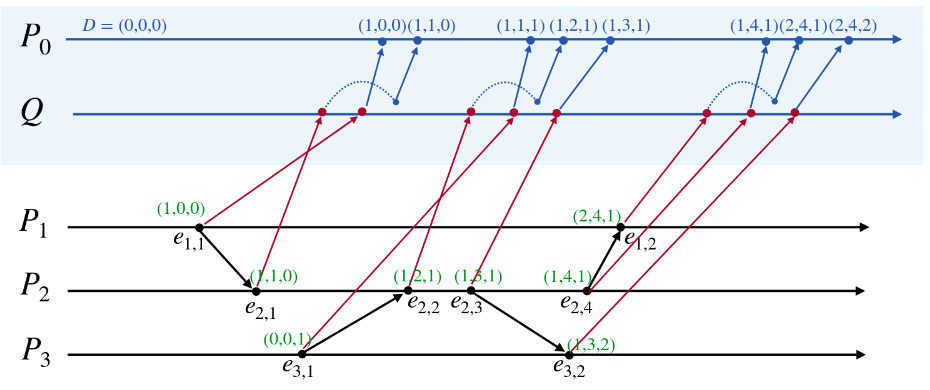
\includegraphics[width=0.5\linewidth]{img/Alg_entrega_causal.png}
  \caption{Algoritmo de entrega causal}\label{fig:1760798568394}
\end{figure}

Desde el punto de vista de $P_0$, comparamos lo siguiente
\[
  D[k]\leq Vc(m)[k]
\]

Seguido a eso, para la causalidad (esto se ve en como se retrasa en la cola el envio de $e_{21}$ con $e_{11}$) para un proceso $P_k$ en Q, observamos todas las dimensiones distintas de K:

\[
  \left[   \underbrace{n_1, n_2, \dots}_{\textcolor{red}{\textbf{Vemos esto}}}, n_k ,\underbrace{\dots,n_{n-1}, n_{n},}_{\textcolor{red}{\textbf{Vemos esto}}}   \right] 
\]

Algo a tener en cuenta y es bastante importante, distintos observadores podrian tener distintos relojes vectoriales \textcolor{red}{(esto es debido a latencias con $P_0$)}


\subsubsection{Estados globales}
Un corte puede tener mensajes en transito. pero denotamos la siguiente caracteristica:
\[
    \text{Corte valido} \neq \text{Corte consistente}
\]
Por lo tanto decimos que, un corte consistente es aquel que un evento sucede antes que otro, es considerado

\subsubsection{Algoritmo de Chandy-Lamport}
Este algoritmo sirve para definir cortes consitentes. Si es grafo tiene ciclos, un proceso puede recibir distintas marcas, de distintos procesos (más adelante definiremos que sucede en estos casos).

\begin{figure}[H]
  \centering
  \captionsetup[subfigure]{labelformat=empty}
  \begin{subfigure}[b]{0.48\textwidth}
    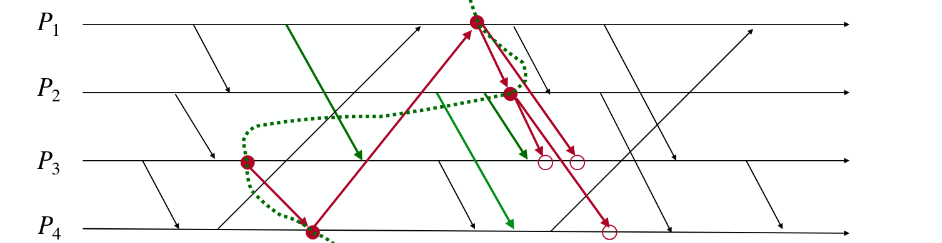
\includegraphics[width=\textwidth]{img/Chandy_ver.png}
    \caption{Visualización del algoritmo}
  \end{subfigure}
  \hspace{2mm} % pequeño espacio entre imágenes
  \begin{subfigure}[b]{0.2\textwidth}
    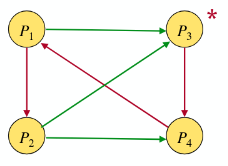
\includegraphics[width=\textwidth]{img/Topologia.png}
    \caption{Topología trabajada}
  \end{subfigure}
  \label{fig:imagenes_lado_a_lado}
\end{figure}

Notar que primero, los nodos que estan totalmente en rojo, son los que por primera vez reciben la marca, por lo tanto, este envia otra marca a sus nodos vecinos. Mientras que las que solo tienen el contorno rojo, y el centro blanco son las que ya recibieron una marca, por ende, no envian una marca.

En casos de ciclos, el algoritmo si termina, dado que, cada nodo manda una marca exactamente, independiente de la cantidad de marcas que vaya a recibir. 

\subsubsection{Estados estables}

Para cualquier estado \textcolor{red}{\textbf{S}} y un estado futuro \textcolor{red}{\textbf{S'}}, si la propiedad \textcolor{red}{\textbf{P}} es verdadera en \textcolor{red}{\textbf{S}}, y el sistema puede llegar a \textcolor{red}{\textbf{S'}}, entonces la propiedad \textcolor{red}{\textbf{P}} tambien debe ser verdadera en \textcolor{red}{\textbf{S'}}

Los siguientes son ejemplos de estados estables:
\begin{center}
  \begin{enumerate}
    \item El sistema esta en deadlock
    \item El algoritmo termino
  \end{enumerate}
\end{center}
Una propiedad podria ser un algoritmo que detecte detención.